\chapter{Dalszy rozwój programu}
Projekt posiada podstawową funkcjonalność symulującą atermiczny zanik sygnału luminescencyjnego w skaleniach. Może być rozwinięty i ulepszony o dodatkowe funkcje.

Jak zaobserwowano podczas wykonywania symulacji największą trudnością w działaniu programu jest jego złożoność obliczeniowa, a co za tym idzie czas wykonywania programu. Na chwilę obecną podczas trwania symulacji każdy elektron, który może przetunelować do centrum rekombinacji jest porównywany ze wszystkimi dziurami elektronowymi do czasu spełnienia warunku zajścia efektu tunelowego \ref{eq:1}. Oznacza to, że elektron traktuje każdą dziurę na równi z innymi dziurami. Jak wynika ze wzoru \ref{eq:2} na prawdopodobieństwo zajścia efektu tunelowego w znacznym stopniu wpływa odległość między pułapką z elektronem, a centrum rekombinacji. Dlatego też przy dalszym rozwoju programu należy zoptymalizować kod w taki sposób, aby dziury znajdujące się bliżej elektronu miały wyższy priorytet przy wyliczaniu prawdopodobieństwa tunelowania tzn. były rozważane wcześniej niż dziury odległe. 

Jednym z pomysłów takiej optymalizacji jest użycie drzewa \emph{kd} (w tym przypadku k = 3) czyli podział kryształu skalenia na \emph{N} regiony. Dla każdego elektronu oraz każdej dziury przechowywana byłaby dodatkowa informacja na temat ich przynależności do danego regionu, określana na podstawie współrzędnych cząstki. Gdy dla danego elektronu rozważane byłoby prawdopodobieństwo zajścia efektu tunelowego, do jego wyliczenia w pierwszej kolejności wybierane zostaną dziury uwięzione w tym samym regionie. Jeśli efekt tunelowania nie zaszedł to w zależności od dalszej implementacji program mógłby uznać, że dla tej iteracji elektron nie będzie tunelował lub kontynuowałby sprawdzanie prawdopodobieństwa w sąsiadujących regionach.

Jak zaobserwowano na wykresach w rozdziale \hyperref[wynik:wykres]{4} na początku działania symulacji otrzymano znaczny spadek ilości wzbudzonych elektronów, a dopiero potem wykres kształtem przypomina funkcję liniową. Jest to spowodowane losowym ustalaniem współrzędnych cząstek, przez co przy starcie programu część elektronów znajduje się bardzo blisko dziur umożliwiając zajście efektu tunelowego. Aby ulepszyć otrzymywany wykres, należałoby zaimplementować funkcję, która będzie monitorowała zapisywanie wyników tak, aby pod uwagę brane były tylko dane po początkowym spadku ilości elektronów wynikającym z losowych współrzędnych startowych. Przykładowy wykres wyglądałby wtedy następująco:
\begin{figure}[h]
\centering
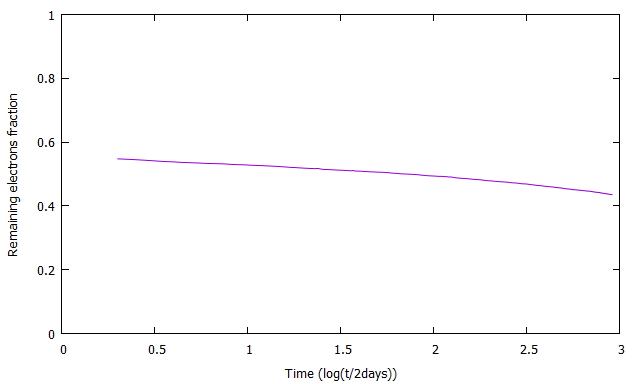
\includegraphics[width=17cm]{przyklad_ulepszony}
\end{figure}

Inną możliwością rozbudowy programu jest dodanie nowej funkcjonalności. Obecnie kroki czasowe przy sprawdzaniu prawdopodobieństwa zajścia tunelowania są równe. Z funkcji prawdopodobieństwa tunelowania wynika, że dobrym pomysłem byłoby wykorzystanie kroków logarytmicznych - na początku działania symulacji używane są małe przedziały czasowe np. sekundy, następnie minuty, potem godziny, dni, lata, dziesiątki lat itd.

Aby program dostarczał bardziej miarodajne dane, należałoby również umożliwić elektronom wielokrotne tunelowanie. W obecnej implementacji elektron po przetunelowaniu nie jest brany pod uwagę w kolejnej iteracji przy wyliczaniu prawdopodobieństwa zajścia tego efektu. W rzeczywistym krysztale zdarza się jednak, że ten sam elektron może tunelować większą ilość razy.

Istnieje również możliwość łatwej zmiany kodu w celu użycia różnych wzorów na prawdopodobieństwo zajścia efektu tunelowego oraz zmiany sposobu rozkładu ładunków podczas tworzenia obiektu kryształu. Obecnie używany jest rozkład jednostajny ciągły, lecz nic nie stoi na przeszkodzie zmiany go na np. rozkład Gaussa. 